\documentclass[12pt,a4paper]{article}
\usepackage[utf8]{inputenc}
\usepackage[T1]{fontenc}
\usepackage[indonesian]{babel}
\usepackage{lmodern}
\usepackage{geometry}
\usepackage{amsmath,amssymb,booktabs,array,graphicx,float}
\usepackage{algorithm}
\usepackage{algpseudocode}
\usepackage{listings}
\usepackage{microtype}
\usepackage[hidelinks]{hyperref}
\geometry{margin=2.54cm}
\graphicspath{{../hasil/}{hasil/}}   % lokal: ../hasil/; Overleaf: hasil/ di samping soal1.tex
\newcommand{\R}{\mathbb{R}}
\newcommand{\T}{\mathsf{T}}
% \input biasa di dalam tabular gagal bila diikuti \bottomrule; pakai primitif \@@input
\makeatletter\newcommand{\isitabel}[1]{\@@input #1 }\makeatother

% Penomoran mengikuti nomor bagian: Tabel 2.1, Gambar 6.1, Kode 5.1, persamaan (3.1)
\numberwithin{equation}{section}
\counterwithin{table}{section}
\counterwithin{figure}{section}
\counterwithin{algorithm}{section}
\floatname{algorithm}{Kode}
\setlength{\belowcaptionskip}{6pt}   % jarak antara caption (di atas) dan tabel
\algrenewcommand\algorithmicrequire{\textbf{Masukan:}}
\algrenewcommand\algorithmicensure{\textbf{Keluaran:}}
\lstset{language=Python, basicstyle=\ttfamily\scriptsize, breaklines=true, columns=fullflexible,
  keepspaces=true, showstringspaces=false, frame=single}

\title{Laporan Teknis TK 1 Analisis Numerik\\[3pt]
\large Soal 1: Analisis Perpindahan Penumpang Antarhalte}
\author{Kelompok: \underline{\hspace{4cm}}\\[5pt]
Anggota dan NPM: \underline{\hspace{8cm}}}
\date{Semester Gasal 2026/2027}

\begin{document}
\maketitle

% Rangkuman, Daftar Isi, dan Bagian 1 (Pendahuluan) ditulis kemudian.
\setcounter{section}{1}

%======================================================================
\section{Data dan Validasi}\label{sec:data}

\subsection{Deskripsi data}
Sebuah koridor memiliki $N$ halte bernomor $1,\dots,N$ sesuai urutan lokasinya. Misalkan $X_k$ adalah halte tempat
seorang penumpang berada pada interval waktu ke-$k$. Matriks transisi $T\in\R^{N\times N}$ berisi
$T_{ij}=\Pr(X_{k+1}=j\mid X_k=i)$, yaitu peluang penumpang berpindah dari halte $i$ ke halte $j$ dalam satu interval.
Data kode B terdiri atas enam berkas \texttt{T\_N.csv} untuk $N\in\{16,32,64,128,256,512\}$, masing-masing berisi
$N$ baris dan $N$ kolom bilangan riil tanpa header. Pada keenam berkas, elemen tak-nol hanya terletak pada kolom
$j\in\{i-1,i,i+1,i+2\}$. Dalam satu interval, penumpang hanya dapat mundur satu halte, tetap, atau maju satu hingga dua
halte, sehingga setiap baris memuat dua sampai empat elemen tak-nol dan $T$ berstruktur pita (\emph{banded}).

\subsection{Prosedur validasi}
Setiap matriks dibaca dengan fungsi \texttt{baca\_T} lalu diperiksa oleh \texttt{validasi\_T}
(Lampiran~\ref{lamp:kode}). Pemeriksaan pertama menyangkut bentuk data: $T$ harus berukuran $N\times N$ sesuai nama
berkas, seluruh elemennya hingga (bukan NaN atau Inf), dan $T_{ij}\ge0$ karena setiap elemen adalah peluang.
Jumlah setiap baris harus satu. Data disimpan sebagai bilangan titik-mengambang, jadi syarat ini diperiksa dengan
toleransi, yaitu $\max_i\bigl\lvert\sum_{j=1}^{N}T_{ij}-1\bigr\rvert\le\tau$ dengan $\tau=10^{-12}$. Nilai $\tau$
jauh di atas epsilon mesin presisi ganda, $\varepsilon=2^{-53}\approx1.11\times10^{-16}$~\cite{heath}, tetapi cukup
kecil untuk mendeteksi kesalahan data.

Syarat berikutnya menjamin distribusi \emph{steady state} tunggal. Rantai Markov berhingga yang \emph{irreducible},
yaitu setiap halte dapat dicapai dari setiap halte lain, memiliki tepat satu distribusi stasioner dan seluruh
komponennya positif~\cite{norris}. Untuk memeriksanya, $T$ dipandang sebagai graf berarah $G$ dengan simpul berupa
halte dan sisi $i\to j$ jika $T_{ij}>0$. Rantai irreducible jika dan hanya jika $G$ terhubung kuat. Hal ini
diperiksa dengan dua \emph{breadth-first search} (BFS)~\cite{cormen} dari halte~1. BFS pertama dijalankan pada $G$
untuk memastikan semua halte dapat dicapai dari halte~1, dan BFS kedua pada $G$ dengan arah sisi dibalik untuk
memastikan halte~1 dapat dicapai dari semua halte. Sebagai pemeriksaan tambahan, rantai juga harus aperiodik agar
distribusi penumpang konvergen ke distribusi stasioner dari kondisi awal apa pun~\cite{norris}. Untuk rantai
irreducible, cukup ada satu $T_{ii}>0$. Karena $T$ disimpan dense, setiap BFS memindai satu baris atau kolom penuh
untuk setiap simpul, sehingga biaya validasi $O(N^2)$. Biaya ini termasuk tahap persiapan data, bukan solver.

\subsection{Hasil validasi}\label{subsec:hasilvalidasi}
\begin{table}[H]
\centering
\caption{Hasil validasi matriks transisi. Untuk semua $N$, dimensi sesuai, seluruh elemen hingga dan nonnegatif,
rantai irreducible dan aperiodik, dan setiap baris memuat 2--4 elemen tak-nol.}
\label{tab:validasi}
\begin{tabular}{rcccc}
\toprule
$N$ & $\max_i\lvert\sum_j T_{ij}-1\rvert$ & $\min_i T_{ii}$ & $\min\{T_{ij}>0: i\ne j\}$ & Valid\\
\midrule
\isitabel{generated/tabel_validasi.tex}
\bottomrule
\end{tabular}
\end{table}

Tabel~\ref{tab:validasi} menunjukkan bahwa keenam matriks lolos seluruh pemeriksaan. Galat jumlah baris maksimum
adalah $\varepsilon$ untuk $N=16$ dan $2\varepsilon=2.22\times10^{-16}$ untuk ukuran lainnya, jadi selisih tersebut
berasal dari pembulatan dan bukan dari kesalahan data. Seluruh elemen diagonal bernilai paling sedikit $0.835$,
sehingga setiap rantai aperiodik. Setiap $T$ karena itu memiliki distribusi stasioner tunggal yang positif di semua
halte. Sifat irreducible ini juga menjadi dasar bahwa matriks koefisien pada Bagian~\ref{sec:formulasi} nonsingular.
Fungsi validasi juga diuji pada empat matriks $3\times3$, yaitu satu matriks valid dan tiga matriks yang sengaja
dibuat salah (ada elemen negatif, satu baris berjumlah $0.9$, dan satu halte menyerap sehingga rantai tidak
irreducible). Keempat keputusan sesuai harapan (\texttt{hasil/uji\_validasi.csv}), jadi fungsi tersebut tidak sekadar
meloloskan semua data.

Kolom keempat Tabel~\ref{tab:validasi} memperlihatkan satu pengecualian. Pada $N=256$, peluang pindah antara halte 128
dan 129 hanya berorde $10^{-8}$, sedangkan peluang pindah positif terkecil pada matriks lain sekitar $0.014$. Total
peluang lintas dari halte 1--128 ke halte 129--256, yaitu $\sum_{i\le128<j}T_{ij}$, hanya sekitar
$9.0\times10^{-8}$, dan arah sebaliknya juga sekitar $9.0\times10^{-8}$. Matriks $T_{256}$ tetap valid karena peluang
itu positif dan rantai tetap irreducible. Namun, koridornya hampir terpecah menjadi dua blok. Dampaknya terhadap
kondisi sistem linear dibahas pada Bagian~7.

%======================================================================
\section{Formulasi dan Penanganan Singularitas}\label{sec:formulasi}
Misalkan $\pi^{(k)}\in\R^N$ adalah vektor kolom dengan $\pi^{(k)}_i=\Pr(X_k=i)$. Hukum peluang total memberi
$\pi^{(k+1)}_j=\sum_{i}\pi^{(k)}_i T_{ij}$, atau $\pi^{(k+1)}=T^\T\pi^{(k)}$. Distribusi steady state
$\pi$ adalah distribusi yang tidak berubah oleh satu langkah transisi, sehingga memenuhi
\begin{equation}\label{eq:steady}
T^\T\pi=\pi,\qquad \mathbf1^\T\pi=1,\qquad \pi_i\ge0,
\end{equation}
dengan $\mathbf1\in\R^N$ vektor yang seluruh elemennya satu. Dengan mendefinisikan $A=I-T^\T$, persamaan pertama
menjadi $A\pi=0$.

Matriks $A$ singular. Setiap baris $T$ berjumlah satu, yaitu $T\mathbf1=\mathbf1$, sehingga
\[
\mathbf1^\T A=\mathbf1^\T-(T\mathbf1)^\T=\mathbf0^\T .
\]
Jumlah seluruh baris $A$ adalah vektor nol. Baris-baris $A$ bergantung linear dan $\det A=0$, jadi eliminasi Gauss
atau faktorisasi LU tidak dapat langsung dipakai pada $A$. Hubungan yang sama menunjukkan bahwa baris pertama $A$
sama dengan $-\sum_{i\ge2}A_{i,:}$. Persamaan pertama dari $A\pi=0$ tidak membawa informasi baru~\cite{stewart}, dan
dapat diganti dengan syarat skala $z_1=1$:
\begin{equation}\label{eq:B}
B_{1,:}=e_1^\T,\qquad B_{i,:}=A_{i,:}\ (i=2,\dots,N),\qquad b=e_1,\qquad Bz=b,
\end{equation}
dengan $e_1=(1,0,\dots,0)^\T$.

Matriks $B$ nonsingular. Ekspansi kofaktor sepanjang baris pertama memberi $\det B=\det A_{2:N,2:N}$, yaitu
determinan $A$ setelah baris dan kolom halte~1 dibuang. Submatriks ini sama dengan $I-\widetilde T^\T$, dengan
$\widetilde T$ matriks transisi tanpa halte~1. Karena rantai irreducible, penumpang di halte mana pun pada akhirnya
mencapai halte~1. Peluang untuk terus berada di halte $2,\dots,N$ menuju nol, yaitu $\widetilde T^k\to0$. Akibatnya
1 bukan nilai eigen $\widetilde T$, sehingga $I-\widetilde T^\T$ dan $B$ nonsingular~\cite{stewart}.

Solusi $z$ masih perlu dinormalkan. Distribusi tunggal $\pi$ memenuhi $A_{i,:}\pi=0$ untuk $i\ge2$ dan $\pi_1>0$,
jadi solusi tunggal $Bz=b$ adalah $z=\pi/\pi_1$. Baris pertama hanya memilih skala $z_1=1$, sehingga umumnya
$\mathbf1^\T z\ne1$. Normalisasi
\begin{equation}\label{eq:normal}
\pi=\frac{z}{\mathbf1^\T z}
\end{equation}
mengembalikan syarat $\mathbf1^\T\pi=1$. Syarat $\pi_i\ge0$ ikut terpenuhi karena $z=\pi/\pi_1>0$.

%======================================================================
\section{Identifikasi Struktur Banded}\label{sec:band}
Untuk matriks $M\in\R^{N\times N}$, \emph{lower bandwidth} $p$ dan \emph{upper bandwidth} $q$ adalah
\begin{equation}\label{eq:pq}
p=\max\{\,i-j : M_{ij}\ne0\,\},\qquad q=\max\{\,j-i : M_{ij}\ne0\,\},
\end{equation}
dengan nilai $0$ jika himpunannya kosong. Matriks pita hanya memiliki elemen tak-nol pada $p$ diagonal di bawah dan
$q$ diagonal di atas diagonal utama. Fungsi \texttt{deteksi\_bandwidth} menghitung~\eqref{eq:pq} secara otomatis dari
posisi elemen tak-nol. Untuk keenam ukuran diperoleh $p=2$ dan $q=1$, baik untuk $A$ maupun $B$. Jadi $B$
\emph{bukan} tridiagonal.

Struktur ini dapat diturunkan langsung. Untuk $i\ge2$, $B_{ij}=\delta_{ij}-T_{ji}$ dengan $\delta_{ij}$ delta
Kronecker, sehingga elemen tak-nol $T$ pada posisi $j-i=d$ muncul di $B$ pada posisi $j-i=-d$. Karena posisi tak-nol
$T$ adalah $d\in\{-1,0,1,2\}$, baris $i\ge2$ dari $B$ hanya memuat
\begin{equation}\label{eq:bandB}
B_{i,i-2}=-T_{i-2,i},\quad B_{i,i-1}=-T_{i-1,i},\quad B_{ii}=1-T_{ii},\quad B_{i,i+1}=-T_{i+1,i}.
\end{equation}
Penggantian baris pertama dengan $e_1^\T$ tetap mempertahankan struktur pita. Vektor $e_1^\T$ hanya tak-nol pada
diagonal, jadi penggantian itu dapat menghapus elemen tak-nol tetapi tidak pernah menambah elemen di luar pita.

Matriks dense membutuhkan $N^2$ bilangan, sedangkan pita $B$ hanya $(p+q+1)N$. Solver dengan \emph{partial pivoting}
membutuhkan sedikit ruang tambahan. Pertukaran baris $k$ dengan baris $r\le k+p$ membawa elemen tak-nol sampai kolom
$r+q\le k+p+q$, sehingga upper bandwidth faktor $U$ dapat naik dari $q$ menjadi $p+q$ (\emph{fill-in}), sementara
lower bandwidth $L$ tetap $p$~\cite{golub}. Kami menyimpan $B$ dalam array $AB\in\R^{(2p+q+1)\times N}$ dengan format
penyimpanan pita LAPACK~\cite{lapack}: $B_{ij}$ berada di $AB_{\,p+q+1+i-j,\;j}$, sehingga setiap diagonal $B$ menjadi
satu baris $AB$ dan $p$ baris teratas dicadangkan untuk fill-in. Untuk $p=2$ dan $q=1$, array ini berukuran
$6\times N$.

\begin{table}[H]
\centering
\caption{Kebutuhan memori penyimpanan $B$ dalam byte (\texttt{float64}, 8 byte per elemen): dense $N^2$,
pita $(p+q+1)N$, dan pita dengan ruang fill-in $(2p+q+1)N$. Rasio = dense dibagi pita dengan fill-in.}
\label{tab:storage}
\begin{tabular}{rrrrr}
\toprule
$N$ & Dense & Pita & Pita + fill-in & Rasio\\
\midrule
\isitabel{generated/tabel_storage.tex}
\bottomrule
\end{tabular}
\end{table}

Tabel~\ref{tab:storage} menunjukkan bahwa rasio penyimpanan dense terhadap pita dengan ruang fill-in sama dengan
$N/6$. Keunggulan penyimpanan pita tumbuh linear terhadap $N$. Pada $N=512$, matriks dense membutuhkan 2 MiB,
sedangkan pita hanya 24 KiB, atau sekitar 85 kali lebih kecil.

%======================================================================
\section{Metode Penyelesaian}\label{sec:metode}
Kedua solver diimplementasikan sendiri dalam \texttt{soal1/soal1.ipynb}. NumPy hanya dipakai untuk array,
\emph{indexing}, dan aritmetika dasar; tidak ada pustaka penyelesaian SPL atau faktorisasi di dalam solver.
Fungsi \texttt{np.linalg.solve} hanya dipakai pada sel verifikasi yang diberi label terpisah. Matriks permutasi $P$
disimpan sebagai vektor indeks.

\subsection{LU dense dengan partial pivoting}
Solver (a) menghitung $PB=LU$ dengan $L$ segitiga bawah berdiagonal satu, $U$ segitiga atas, dan $P$ matriks
permutasi~\cite{heath}. Pada langkah $k$, baris dengan $\lvert B_{ik}\rvert$ terbesar ($i\ge k$) ditukar ke posisi
$k$. Pertukaran dilakukan pada seluruh baris, termasuk multiplier yang sudah tersimpan, agar $L$ konsisten dengan $P$
akhir. Multiplier $\ell_{ik}=B_{ik}/B_{kk}$ disimpan di tempat elemen yang dieliminasi, sehingga $L$ dan $U$ berbagi
satu array $N\times N$. Sistem kemudian diselesaikan dengan substitusi maju $Ly=Pb$ dan substitusi mundur $Uz=y$.
Langkah-langkah ini dirangkum pada Kode~\ref{alg:dense} dan diimplementasikan pada fungsi \texttt{lu\_dense} dan
\texttt{solve\_lu}.

\begin{algorithm}[H]
\caption{LU dense dengan \emph{partial pivoting} dan penyelesaian $Bz=b$}
\label{alg:dense}
\begin{algorithmic}[1]
\Require $B\in\R^{N\times N}$ nonsingular, $b\in\R^N$
\Ensure $z\in\R^N$ dengan $Bz=b$
\State $M\gets B$ (salinan); $\mathit{perm}\gets(1,2,\dots,N)$
\For{$k=1$ \textbf{to} $N-1$}
  \State $r\gets\arg\max_{k\le i\le N}\lvert M_{ik}\rvert$; \textbf{if} $M_{rk}=0$ \textbf{then error} ``singular''
  \State Tukar baris $M_{k,:}\leftrightarrow M_{r,:}$ dan $\mathit{perm}_k\leftrightarrow\mathit{perm}_r$
  \Comment{seluruh baris}
  \For{$i=k+1$ \textbf{to} $N$}
    \State $M_{ik}\gets M_{ik}/M_{kk}$ \Comment{multiplier $\ell_{ik}$}
    \State $M_{i,k+1:N}\gets M_{i,k+1:N}-M_{ik}\,M_{k,k+1:N}$
  \EndFor
\EndFor
\State $y\gets b_{\mathit{perm}}$ \Comment{$y=Pb$}
\For{$i=2$ \textbf{to} $N$} \Comment{substitusi maju $Ly=Pb$}
  \State $y_i\gets y_i-\sum_{j<i}M_{ij}y_j$
\EndFor
\For{$i=N$ \textbf{downto} $1$} \Comment{substitusi mundur $Uz=y$}
  \State $z_i\gets\bigl(y_i-\sum_{j>i}M_{ij}z_j\bigr)/M_{ii}$
\EndFor
\State \Return $z$
\end{algorithmic}
\end{algorithm}

\subsection{Solver banded bergaya Thomas}
Solver (b) harus berjalan dalam $O(N)$ waktu dan memori. Algoritma Thomas klasik memenuhi syarat ini, tetapi hanya
berlaku untuk matriks tridiagonal ($p=q=1$), sedangkan $B$ memiliki $p=2$ dan $q=1$. Solver (b) karena itu berupa
perluasannya untuk matriks pita umum, yaitu eliminasi Gauss dengan partial pivoting yang hanya bekerja di dalam
pita~\cite{golub}, langsung pada array $AB$ dari Bagian~\ref{sec:band}. Algoritmanya ada pada Kode~\ref{alg:band} (fungsi \texttt{bentuk\_B\_band},
\texttt{lu\_band}, dan \texttt{solve\_band}).

Ada tiga hal yang membuat solver ini berjalan dalam $O(N)$. Pertama, pita diambil langsung dari $T$: fungsi
\texttt{bentuk\_B\_band} mengisi $AB$ menurut~\eqref{eq:bandB} dan hanya mengakses $N(p+q+1)$ elemen $T$, jadi
matriks $B$ dense, $L$, $U$, maupun $P$ berukuran $N\times N$ tidak pernah dibentuk. Kedua, pivot hanya dicari di
baris $k,\dots,\min(N,k+p)$ karena di bawahnya kolom $k$ sudah nol, sedangkan pertukaran dan pembaruan hanya
menyentuh kolom $k,\dots,\min(N,k+p+q)$. Ketiga, multiplier langkah sebelumnya tidak ikut ditukar seperti pada
Kode~\ref{alg:dense}, karena tersimpan di kolom lain $AB$. Indeks pertukaran setiap langkah dicatat di vektor
$\mathit{piv}$, lalu diulang dengan urutan yang sama pada ruas kanan saat substitusi maju. Hasilnya setara dengan
$PB=LU$.

\begin{algorithm}[H]
\caption{Faktorisasi dan penyelesaian banded dengan \emph{partial pivoting}. Notasi $B_{ij}$ berarti elemen yang
disimpan di $AB_{p+q+1+i-j,\,j}$.}
\label{alg:band}
\begin{algorithmic}[1]
\Require $AB\in\R^{(2p+q+1)\times N}$ berisi pita $B$, $p$, $q$, $b\in\R^N$
\Ensure $z\in\R^N$ dengan $Bz=b$
\For{$k=1$ \textbf{to} $N$}
  \State $i_{\max}\gets\min(N,k+p)$; \quad $j_{\max}\gets\min(N,k+p+q)$
  \State $r\gets\arg\max_{k\le i\le i_{\max}}\lvert B_{ik}\rvert$; \textbf{if} $B_{rk}=0$ \textbf{then error}
  ``singular''
  \State $\mathit{piv}_k\gets r$; tukar $B_{kj}\leftrightarrow B_{rj}$ untuk $j=k,\dots,j_{\max}$
  \For{$i=k+1$ \textbf{to} $i_{\max}$}
    \State $B_{ik}\gets B_{ik}/B_{kk}$ \Comment{multiplier $\ell_{ik}$}
    \State $B_{ij}\gets B_{ij}-B_{ik}B_{kj}$ untuk $j=k+1,\dots,j_{\max}$
  \EndFor
\EndFor
\State $y\gets b$
\For{$k=1$ \textbf{to} $N$} \Comment{maju: ulangi pertukaran dan eliminasi}
  \State tukar $y_k\leftrightarrow y_{\mathit{piv}_k}$; \quad
         $y_i\gets y_i-B_{ik}y_k$ untuk $i=k+1,\dots,\min(N,k+p)$
\EndFor
\For{$i=N$ \textbf{downto} $1$} \Comment{mundur: $U$ selebar $p+q$}
  \State $z_i\gets\bigl(y_i-\sum_{j=i+1}^{\min(N,i+p+q)}B_{ij}z_j\bigr)/B_{ii}$
\EndFor
\State \Return $z$
\end{algorithmic}
\end{algorithm}

\subsection{Uji kebenaran}
Sebelum dipakai pada data, kedua solver diuji pada matriks kecil yang hasilnya dapat dicek manual
(Tabel~\ref{tab:uji}). Pada uji~2, hitungan tangan dengan dua kali pertukaran baris memberi
\[
L=\begin{pmatrix}1&0&0\\0.25&1&0\\0.5&2/3&1\end{pmatrix},\qquad
U=\begin{pmatrix}8&7&9\\0&-0.75&-1.25\\0&0&-2/3\end{pmatrix},\qquad
\mathit{perm}=(3,1,2),
\]
dengan $\mathit{perm}$ urutan baris $B$ setelah permutasi $P$. Kedua solver menghasilkan faktor yang sama persis.

\begin{table}[H]
\centering
\caption{Uji kebenaran pada matriks kecil.}
\label{tab:uji}
\small
\begin{tabular}{@{}>{\raggedright}p{0.34\textwidth}>{\raggedright}p{0.12\textwidth}>{\raggedright\arraybackslash}p{0.44\textwidth}@{}}
\toprule
Kasus & Solver & Hasil\\
\midrule
1. Matriks valid dan tiga matriks rusak $3\times3$ (Bagian~\ref{sec:data}) & validasi & keempat keputusan sesuai\\
2. $B=\left(\begin{smallmatrix}2&1&1\\4&3&3\\8&7&9\end{smallmatrix}\right)$, $b=(3,7,19)^\T$
   & dense, banded ($p=q=2$) & $L$, $U$, $P$ sama dengan hitungan tangan; $\max\lvert PB-LU\rvert=0$;
   $z=(1,-1,2)^\T$\\
3. Matriks $4\times4$ dengan $B_{11}=0$ & dense & baris 1 dan 2 ditukar; galat solusi $4.4\times10^{-16}$\\
4. Matriks pita $8\times8$, $p=2$, $q=1$, diagonal diperkecil 100 kali & banded vs dense & 7 pertukaran baris,
   8 elemen fill-in, $U$ melebar tepat sampai $p+q=3$; $P$ dan $U$ identik dengan solver dense;
   galat solusi $5.3\times10^{-15}$\\
5. Matriks singular $\left(\begin{smallmatrix}1&2\\2&4\end{smallmatrix}\right)$ & dense, banded &
   keduanya menolak karena pivot nol\\
6. Rantai \emph{birth--death} $3\times3$ dengan $\pi=(\tfrac14,\tfrac12,\tfrac14)^\T$ & dense, banded &
   $\pi$ tepat sama\\
\bottomrule
\end{tabular}
\end{table}

Pada keenam data, pivoting tidak pernah menukar baris (\texttt{hasil/akurasi\_dense.csv} dan
\texttt{hasil/akurasi\_band.csv}). Penyebabnya, $B$ dominan diagonal per kolom. Pada kolom $k\ge2$ berlaku
$\lvert B_{kk}\rvert=1-T_{kk}=\sum_{i\ne k}T_{ki}\ge\sum_{i\ne k,\,i\ge2}\lvert B_{ik}\rvert$, dan pada kolom pertama
$B_{11}=1\ge T_{12}+T_{13}$. Eliminasi Gauss mempertahankan sifat ini, sehingga partial pivoting selalu memilih elemen
diagonal~\cite{golub}. Jalur pertukaran baris karena itu hanya teruji lewat uji~2--4 pada Tabel~\ref{tab:uji}.

Tanpa pertukaran baris, kedua solver melakukan operasi titik-mengambang yang sama pada angka yang sama; solver dense
hanya menambah operasi terhadap elemen nol. Hasilnya, $\pi$ dari solver banded identik dengan $\pi$ dari solver dense,
dengan selisih maksimum tepat $0$ untuk semua $N$. Sebagai pembanding independen, selisih terhadap
\texttt{np.linalg.solve} paling besar $2.6\times10^{-16}$ untuk $N\ne256$ dan $6.6\times10^{-13}$ untuk $N=256$
(\texttt{hasil/verifikasi\_*\_numpy.csv}). Selisih yang lebih besar pada $N=256$ sejalan dengan struktur yang hampir
terpecah pada Subbagian~\ref{subsec:hasilvalidasi} dan dianalisis pada Bagian~7.

%======================================================================
\section{Eksperimen Kinerja dan Analisis Kompleksitas}\label{sec:eksperimen}

\subsection{Rancangan eksperimen}
Eksperimen dijalankan pada AMD Ryzen 7 7435HS dengan RAM 16 GB, Windows 11, Python 3.14.4, dan NumPy 2.5.3.
Waktu solver adalah waktu faktorisasi, substitusi, dan normalisasi~\eqref{eq:normal}. Waktu membaca CSV dan
persiapan diukur terpisah. Persiapan solver dense adalah pembentukan $B$ dense, yang berbiaya $O(N^2)$. Persiapan
solver banded adalah deteksi $p$ dan $q$ dari posisi tak-nol $T$, yang juga $O(N^2)$ karena data masukan dense,
ditambah ekstraksi pita yang $O(N)$. Waktu diukur dengan \texttt{time.perf\_counter}. Setelah satu kali pemanasan,
setiap pengukuran diulang 15 kali dan diambil nilai minimumnya, karena gangguan dari sistem operasi hanya dapat
menambah waktu. Memori diukur dengan dua cara: puncak alokasi selama solver berjalan menurut \texttt{tracemalloc},
dan total \texttt{.nbytes} array yang disimpan solver (koefisien, ruas kanan, faktor, vektor pivot, dan solusi).
Seluruh hasil tersimpan di \texttt{hasil/benchmark.csv}.

\subsection{Hasil}
\begin{table}[H]
\centering
\caption{Waktu (ms, minimum dari 15 ulangan) dan memori (KiB) untuk data soal.}
\label{tab:bench}
\small
\setlength{\tabcolsep}{4pt}
\begin{tabular}{r rrrrr rrrr}
\toprule
 & Baca & \multicolumn{2}{c}{Dense (ms)} & \multicolumn{2}{c}{Banded (ms)} & \multicolumn{2}{c}{\texttt{.nbytes}} &
 \multicolumn{2}{c}{Peak}\\
\cmidrule(lr){3-4}\cmidrule(lr){5-6}\cmidrule(lr){7-8}\cmidrule(lr){9-10}
$N$ & CSV & persiapan & solver & persiapan & solver & dense & banded & dense & banded\\
\midrule
\isitabel{generated/tabel_benchmark.tex}
\bottomrule
\end{tabular}
\end{table}

\begin{figure}[H]
\centering
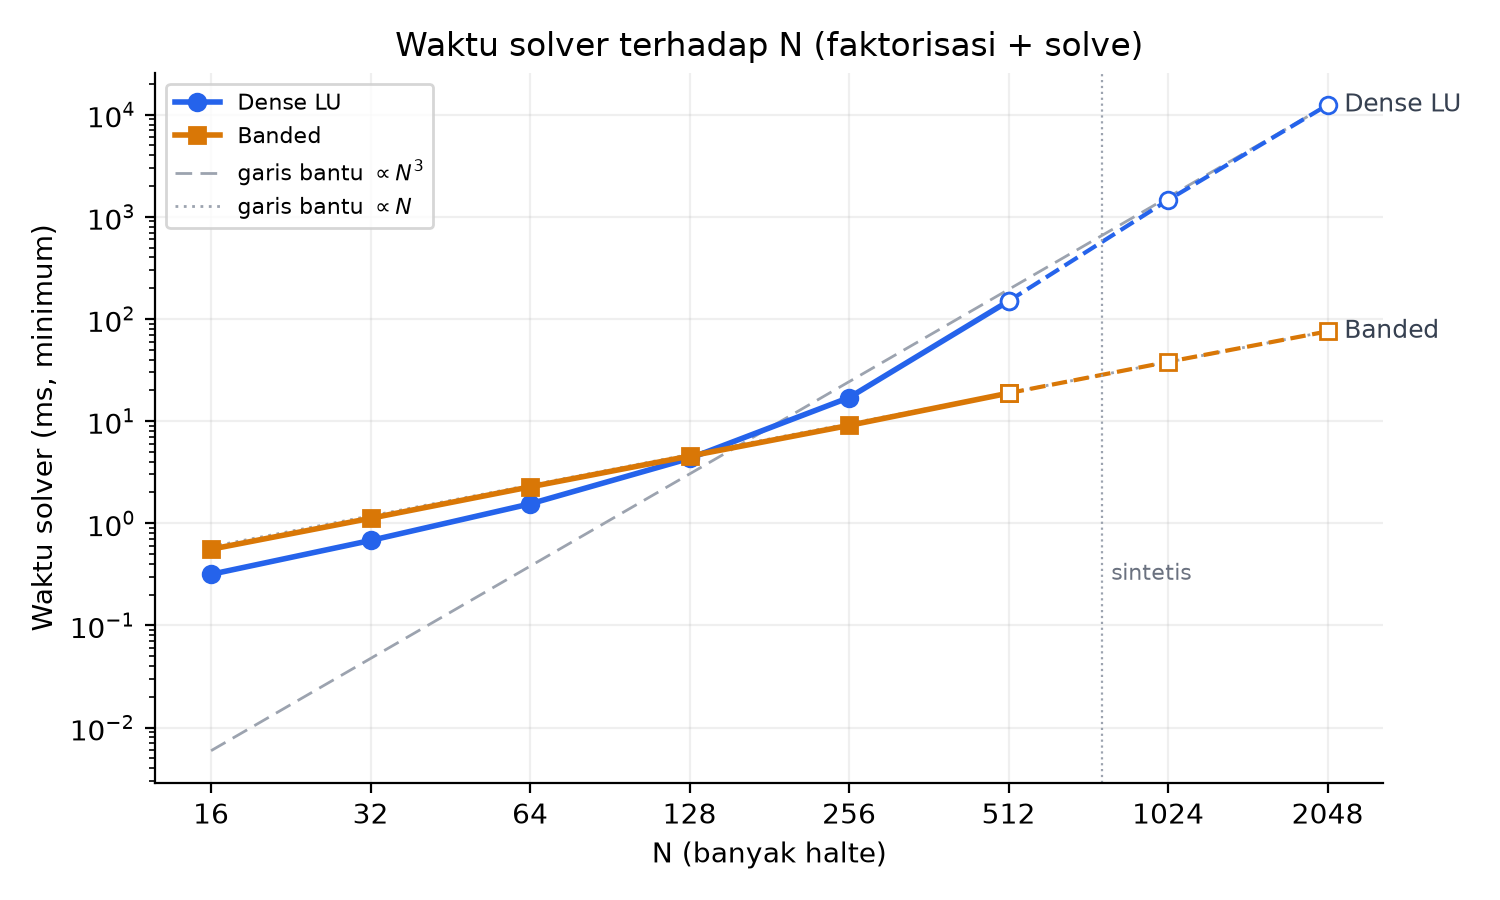
\includegraphics[width=0.78\textwidth]{waktu_vs_N.png}
\caption{Waktu solver terhadap $N$ (skala log--log). Marker kosong dan garis putus-putus adalah rantai sintetis
$N=1024$ dan $2048$; garis abu-abu adalah garis bantu $\propto N^3$ dan $\propto N$.}
\label{fig:waktu}
\end{figure}

Tabel~\ref{tab:bench} dan Gambar~\ref{fig:waktu} menunjukkan bahwa keunggulan solver banded baru muncul pada $N$
sedang. Untuk $N\le64$, solver banded 1.5--1.8 kali lebih lambat daripada solver dense, dan pada $N=128$ keduanya
setara. Setiap langkah solver banded berupa perulangan Python kecil dengan biaya tetap, sedangkan setiap langkah
solver dense adalah satu operasi vektor NumPy yang dieksekusi dalam kode terkompilasi. Pada $N$ kecil, waktu lebih
ditentukan oleh banyaknya langkah daripada banyaknya flop. Mulai $N=256$ solver banded lebih cepat, yaitu 1.9 kali
pada $N=256$ dan 8.0 kali pada $N=512$. Pada $N=512$, waktu membaca CSV (27.1~ms) bahkan sudah melebihi waktu solver
banded (18.8~ms). Untuk melihat tren pada $N$ yang lebih besar, kedua solver juga dijalankan pada rantai sintetis
$N=1024$ dan $2048$ dengan pola pita yang sama (bukan data soal, lima ulangan). Pada $N=2048$, solver dense
membutuhkan 12.4~s, sedangkan solver banded hanya 76~ms.

\begin{figure}[H]
\centering
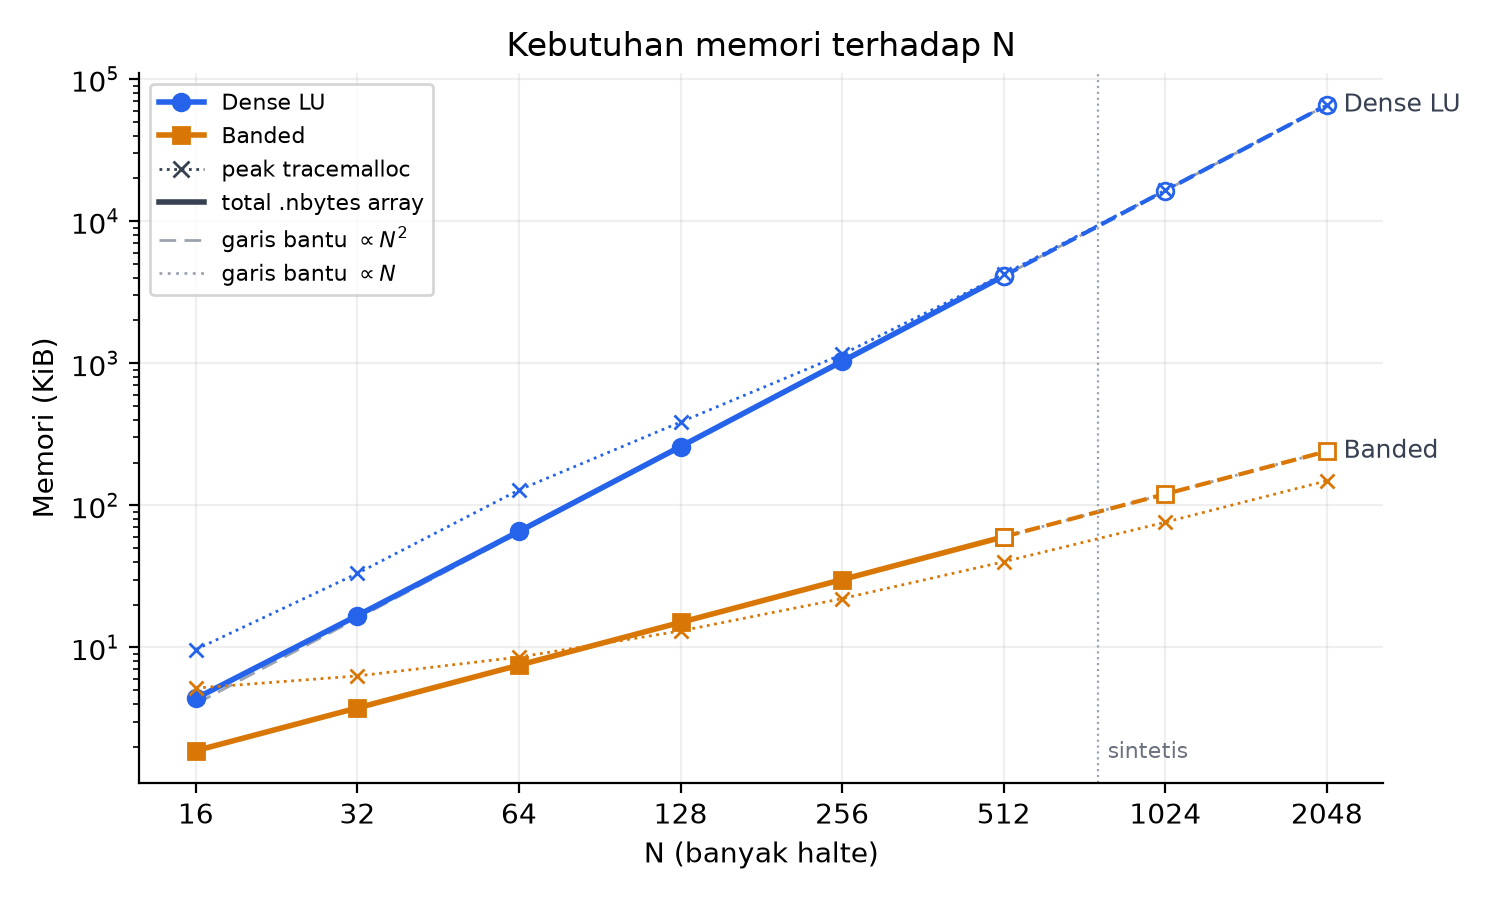
\includegraphics[width=0.78\textwidth]{memori_vs_N.png}
\caption{Memori terhadap $N$. Garis tebal menunjukkan total \texttt{.nbytes} array yang disimpan solver; garis
bertitik dengan marker silang menunjukkan puncak \texttt{tracemalloc}.}
\label{fig:memori}
\end{figure}

Perbedaan memori pada Gambar~\ref{fig:memori} lebih tegas daripada perbedaan waktu. Total \texttt{.nbytes} solver
dense naik empat kali setiap $N$ digandakan, sedangkan solver banded hanya naik dua kali. Pada $N=512$, solver dense
menyimpan 4108~KiB dan solver banded 60~KiB, sekitar 68 kali lebih kecil. Puncak \texttt{tracemalloc} mengikuti pola
yang sama.

\subsection{Analisis kompleksitas}
Banyaknya operasi dihitung dalam flop: satu flop adalah satu pasangan perkalian dan pengurangan, atau satu
pembagian. Pada solver dense, langkah $k$ mengeliminasi $N-k$ baris dan tiap baris memperbarui $N-k$ elemen,
sehingga faktorisasi memerlukan $\sum_{k=1}^{N-1}(N-k)^2\approx N^3/3$ flop~\cite{heath}. Substitusi maju dan
mundur masing-masing sekitar $N^2/2$ flop. Array faktornya berukuran $N^2$. Jadi solver dense membutuhkan $O(N^3)$
waktu dan $O(N^2)$ memori.

Pada solver banded, setiap kolom hanya mengeliminasi $p$ baris, dan setiap baris hanya memperbarui $p+q$ elemen
karena faktor $U$ melebar akibat pivoting. Faktorisasi memerlukan sekitar
\begin{equation}\label{eq:flopband}
N\,p\,(p+q)
\end{equation}
flop, yaitu $6N$ untuk $p=2$ dan $q=1$; taksiran $(p+q)^2N/4$ yang lebih kecil berlaku untuk eliminasi pita tanpa
pivoting. Substitusi maju dan mundur hanya menyentuh elemen di dalam pita, sehingga biayanya $O(N(p+q))$. Memori yang
dibutuhkan adalah array $AB$ berukuran $(2p+q+1)N$. Untuk $p$ dan $q$ tetap, waktu dan memori sama-sama $O(N)$,
sesuai yang dituntut dari solver (b). Sebagai gambaran, pada $N=512$ faktorisasi dense memerlukan sekitar
$4.5\times10^{7}$ flop, sedangkan faktorisasi banded hanya 3072 flop (\texttt{hasil/flop\_teori.csv}).

\begin{table}[H]
\centering
\caption{Kemiringan garis log--log (pangkat empiris $N$) terhadap nilai teoretis. Kolom terakhir memakai
$N=256$, $512$ dan dua titik sintetis.}
\label{tab:slope}
\begin{tabular}{lcccc}
\toprule
Besaran & Teori & $N=16$--$512$ & $N=128$--$512$ & $N=256$--$2048$\\
\midrule
\isitabel{generated/tabel_kemiringan.tex}
\bottomrule
\end{tabular}
\end{table}

Tabel~\ref{tab:slope} membandingkan teori dengan eksperimen melalui kemiringan garis terbaik pada skala log--log,
yang dihitung dengan rumus regresi linear sederhana. Kemiringan waktu solver banded sekitar 1 pada semua rentang,
sesuai $O(N)$. Kemiringan waktu solver dense hanya 1.71 pada seluruh data karena pada $N$ kecil biaya tetap setiap
langkah masih dominan, lalu naik menjadi 2.56 untuk $N\ge128$ dan 3.18 untuk $N\ge256$, mendekati $N^3$. Kemiringan flop
faktorisasi dan \texttt{.nbytes} sama dengan teori: 3 dan 2 untuk dense, 1 untuk banded. Eksperimen ini mengonfirmasi analisis di
atas: solver banded linear dalam waktu dan memori, sedangkan solver dense kuadratik dalam memori dan mendekati kubik
dalam waktu.

%======================================================================
% Bagian 7 (Analisis Kondisi dan Galat), 8, dan 9 ditulis kemudian.

\renewcommand{\refname}{Referensi}
\emergencystretch=1em
\begin{thebibliography}{9}
\bibitem{norris} J. R. Norris, \emph{Markov Chains}. Cambridge University Press, 1997, Bab 1.7--1.8.
\bibitem{cormen} T. H. Cormen, C. E. Leiserson, R. L. Rivest, dan C. Stein, \emph{Introduction to Algorithms},
  edisi ke-3. MIT Press, 2009.
\bibitem{heath} M. T. Heath, \emph{Scientific Computing: An Introductory Survey}, edisi ke-2. McGraw-Hill, 2002,
  Bab 1--2.
\bibitem{stewart} W. J. Stewart, \emph{Introduction to the Numerical Solution of Markov Chains}. Princeton
  University Press, 1994.
\bibitem{golub} G. H. Golub dan C. F. Van Loan, \emph{Matrix Computations}, edisi ke-4. Johns Hopkins University
  Press, 2013, Bab 3 dan Subbab 4.3.
\bibitem{lapack} E. Anderson dkk., \emph{LAPACK Users' Guide}, edisi ke-3. SIAM, 1999.
\end{thebibliography}

\appendix
\section{Kode Program}\label{lamp:kode}
Program lengkap berada di \texttt{soal1/soal1.ipynb} dan dijalankan dengan \emph{Restart \& Run All}; seluruh tabel
dan grafik disimpan ke \texttt{soal1/hasil/}. Berikut fungsi inti validasi, kedua solver, dan pengukuran waktu, disalin
apa adanya dari notebook.
\lstinputlisting{generated/kode_lampiran.py}

\end{document}
